\onehalfspaced

\section{Cost Analysis}

 We have introduced several ways of significantly lowering the costs associated with crowdsourcing translations when a large amount of data are solicited (on the order of millions of samples):
\begin{itemize}
\item We show that after we have collected one translation of a source sentence, we can consult a model that predicts whether its quality is sufficiently high or whether we should pay to have the sentence re-translated.  The cost savings for non-professionals here comes from reducing the number of redundant translations. We can save half of the cost associated with non-professional translations to get 95\% of the translation quality using the full set of redundant translations.
\item We show that we can quickly identify bad translators, either by having them first translate a small number of sentences to be tested against professional translations, or by estimating their performance using a feature-based linear regression model. The cost savings for non-professionals here comes from not hiring bad workers. Similarly, we reduce the non-professional translation cost to the half of the original cost.

\item In both cases we need some amount of professionally translated materials  to use as a gold standard for calibration. Although the unit cost for each reference is much higher than the unit cost for each non-professional translation, the cost associated with non-professional translations can dominate the total cost since the large amount of data need to be collected. Thus, we focus on reducing cost associated with non-professional translations. 
%The cost savings for professionals come from reducing the referencing translations to calibrate each data sample. 
% The cost of these professional translations can dominate the cost of our models, so we experiment with how little we can get away with.
\end{itemize}
%In all cases, there is a trade-off between lowering our costs and producing high quality translations.  Figure \ref{fbleucost} plots the cost versus the BLEU scores for the different configurations that we experimented with.
%
%In Figure \ref{fbleucost}-(a) the increasing costs are a function of how many sentences we use to rank the translators.  Here we use no model, and simply rank the translators by their BLEU score against a small amount of gold standard data. The quality peaks at 37.9 BLEU after \$3,000.
%%the return on investment is low after spending the first \$2,000 to get a BLEU of 35.6.
%We are able to rank the translators with high accuracy and achieve a relative high BLEU score by paying for a comparatively small number of professional translations to use as calibration. From our experiments,  10-20 professionally translated sentences seems like a reasonable number. 
%
%Figure\ref{fbleucost}-(b) uses a model to determine whether to purchase another translation.  
%%Here the starting cost is high (nearly \$9,000) because the model requires a significant amount of professional translations in order to train the model and to determine the optimal threshold values for whether to solicit another translation. 
%This model allows us to significantly improve the overall translation quality to a BLEU score of nearly 40, for a final cost of \$2,700.
%
%%To emphasize the effectiveness of model selection approach, Figure \ref{fbleucost}-(c) plots the relationship between BLEU and non-professional component of the overall cost.  Past approaches to crowdsourcing translation always solicited 4 non-professional translations of every source sentence. The cost for translating our 1433 test sentences under this approach is \$573.44.  This produces the maximum BLEU score of 40.1.  Using our model to reduce the number of redundant translations, we can reduce the costs with mild degredation in translation quality.  We can cut the number of non-translations in half, and pay only \$286.72, while achieving a BLEU score of 37.6 (94\% of the maximum), or pay \$348.36,60.7\% of total non-professional translations' cost, for a BLEU of 38.5 (96\% of  the maximum).
%
%\begin{figure}[htbp]
%  \centering
%  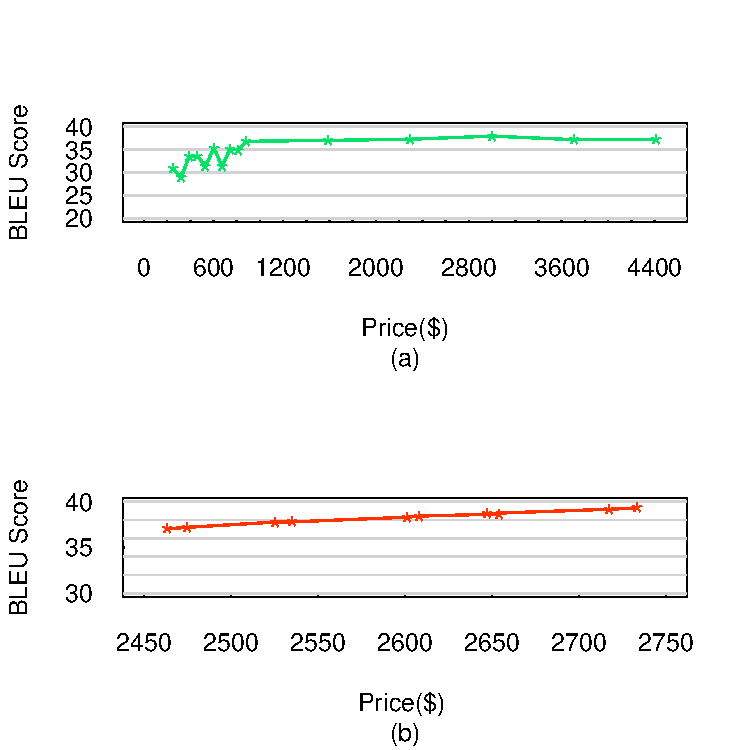
\includegraphics[width=\linewidth]{cost-bleu/pricecost.pdf}
%  \caption{The Relationship between BLEU score and costs. In Figure (a), the red line shows the relationship between BLEU score and  the total costs (professional and non-professional) for the ranking based approach. 
%  %The green line shows the corresponding translation quality for gold standard ranking selection measured in BLEU score. 
%  Figure (b) shows the relationship between BLEU score and the total costs for model-based approach. 
%  %Figure (c)  illustrates the relationship between BLEU score and non-professional costs for model based approach.
%  }
%    \label{fbleucost}
%\end{figure}
